\documentclass[pdflatex,sn-mathphys-num]{sn-jnl}
\usepackage{graphicx,booktabs,amsmath}
\hypersetup{bookmarksdepth=2}
\raggedbottom
\begin{document}
\title{Supplement S1: Source retention for EV charging forecasting}
\author{AIP491\_G10 Research Team}
\maketitle
\section{How to read the complete results}
The three heatmaps below display every method and city group at each initial-history budget. Values are percentage changes in station-macro MAE relative to Fixed retention: negative is lower MAE. Color saturates at $\pm20\%$; printed values are not clipped. These are point estimates, not significance indicators. UrbanEV has 29 scored stations and one retained unscored station; other groups have ten scored sites. Seeds are averaged within station before macro aggregation.

The file \texttt{full-results.csv} contains all 294 method--group--history rows, with original-kWh MAE/RMSE, station counts, negative-transfer rates and the frozen Adaptive-minus-method intervals. Empty interval fields remain undefined. The underlying declared scope is 11,340 method cells, including 126 unscored cells; these aggregate lookup rows are not independent replications. \texttt{switch-audits.csv} preserves the original finite/null audit coverage and signed descriptive statistics. No model was retrained to produce these displays.
\begin{table}[htbp]\centering\small
\caption{Selected Final scope relative to released entity inventories. ``Ready Final'' is the eligible identifier pool for the stated partition and budget, not the raw city population. Percentages refer to selected IDs/raw IDs, not the fraction of all raw records used in Source training.}\label{tab:scope}
\begin{tabular}{@{}lrrrr@{}}\toprule
Namespace & Raw IDs & Ready Final IDs & Selected & Raw share (\%)\\ \midrule
UrbanEV/SZH & 1,682 & 340/341/345 & 30 & 1.78\\
CHARGED/AMS & 2,449 & 478 & 10 & 0.41\\
CHARGED/JHB & 47 & 13 & 10 & 21.28\\
CHARGED/LOA & 229 & 41 & 10 & 4.37\\
CHARGED/MEL & 63 & 15 & 10 & 15.87\\
CHARGED/SPO & 47 & 10 & 10 & 21.28\\
CHARGED/SZH & 1,445 & 271 & 10 & 0.69\\ \botrule
\end{tabular}\end{table}
\clearpage\section{Complete method comparison: 7-day history}\begin{figure}[htbp]\centering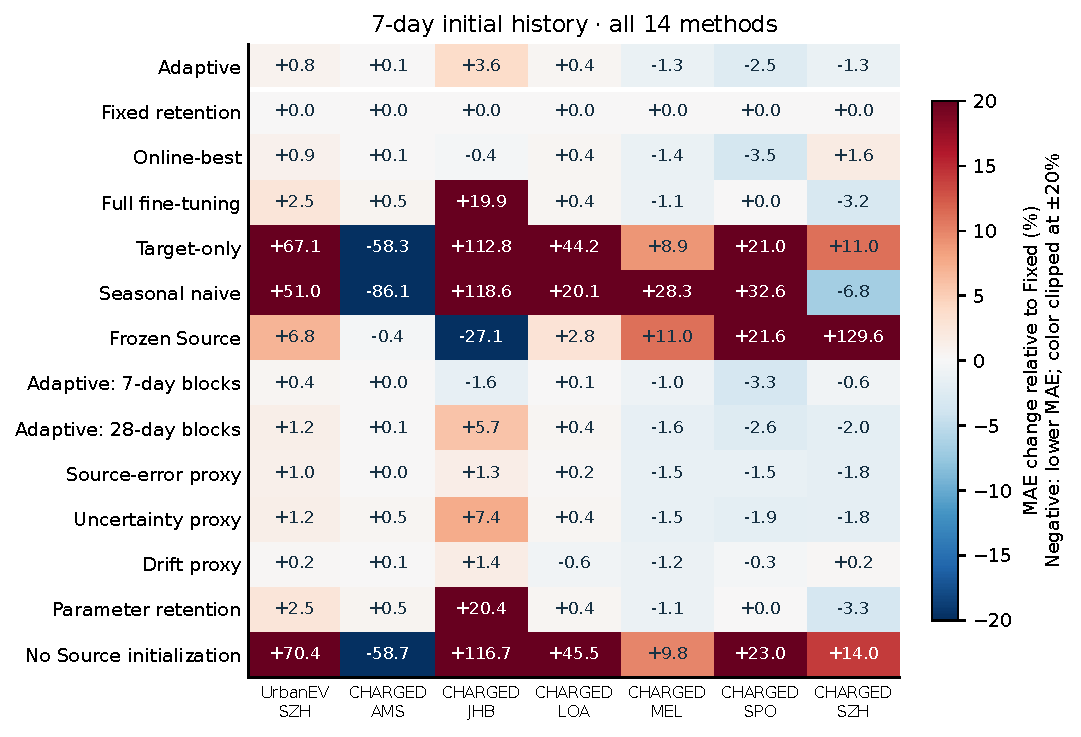
\includegraphics[width=\textwidth]{fig-all-methods-7-v8.pdf}\caption{All 14 methods, 7-day initial history. Refer to the CSV for full-precision absolute MAE and RMSE.}\end{figure}

\clearpage\section{Complete method comparison: 14-day history}\begin{figure}[htbp]\centering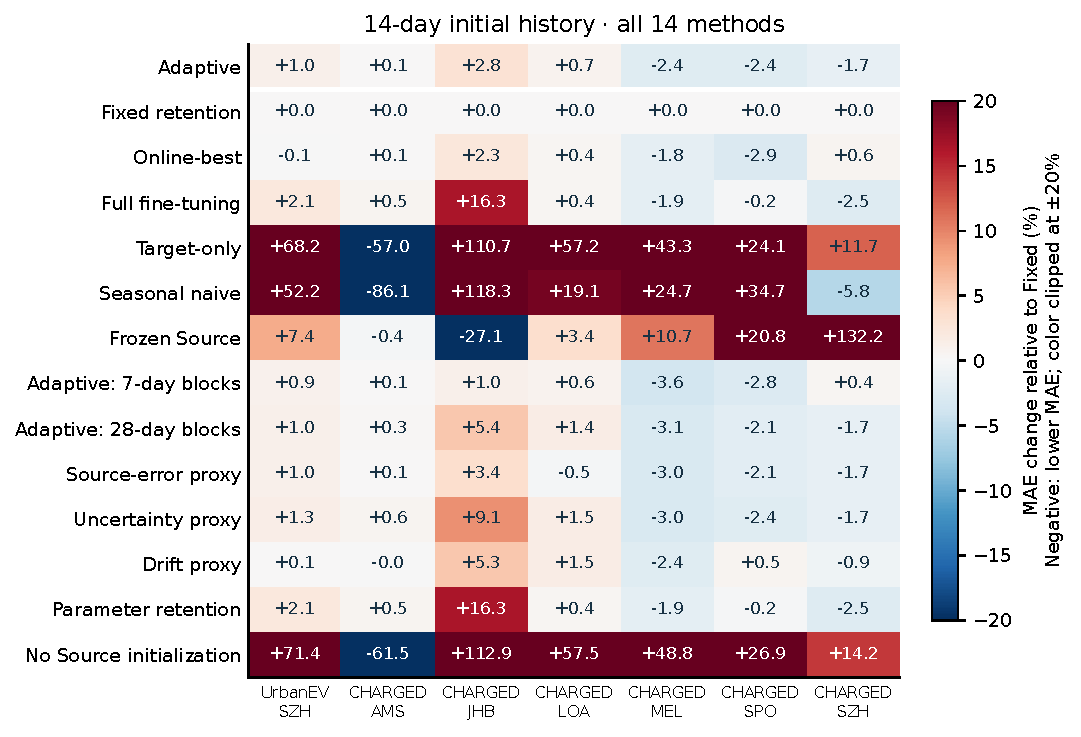
\includegraphics[width=\textwidth]{fig-all-methods-14-v8.pdf}\caption{All 14 methods, 14-day initial history. Refer to the CSV for full-precision absolute MAE and RMSE.}\end{figure}

\clearpage\section{Complete method comparison: 28-day history}\begin{figure}[htbp]\centering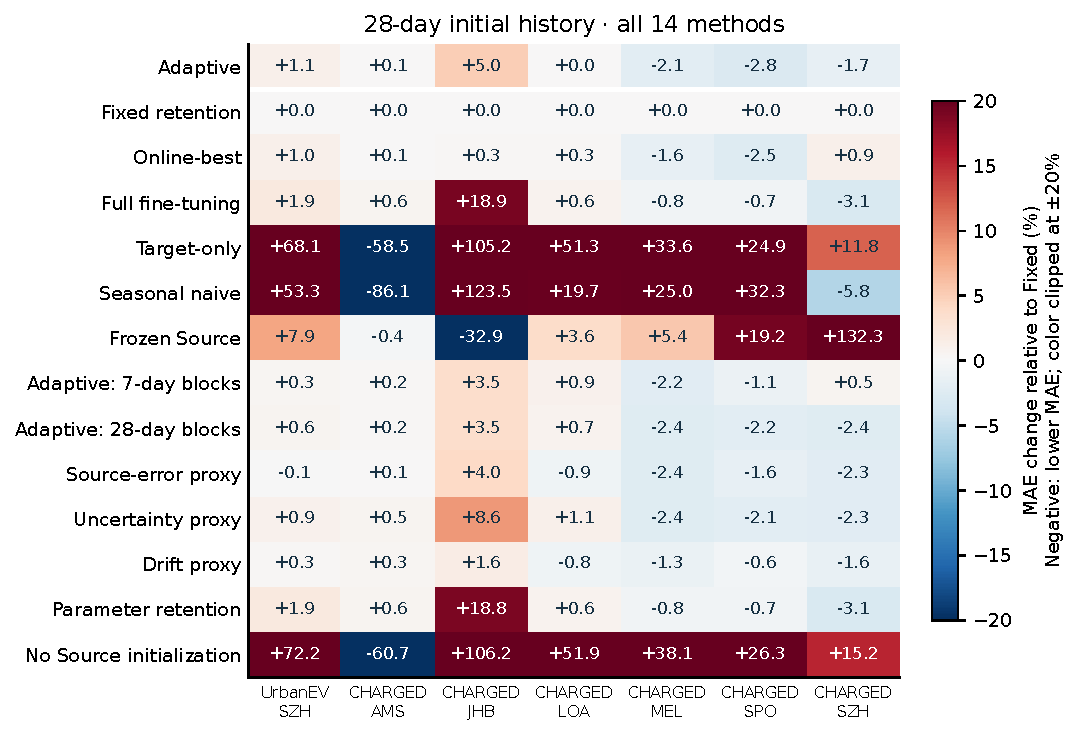
\includegraphics[width=\textwidth]{fig-all-methods-28-v8.pdf}\caption{All 14 methods, 28-day initial history. Refer to the CSV for full-precision absolute MAE and RMSE.}\end{figure}

\clearpage\section{Exploratory uncertainty}
\begin{figure}[htbp]\centering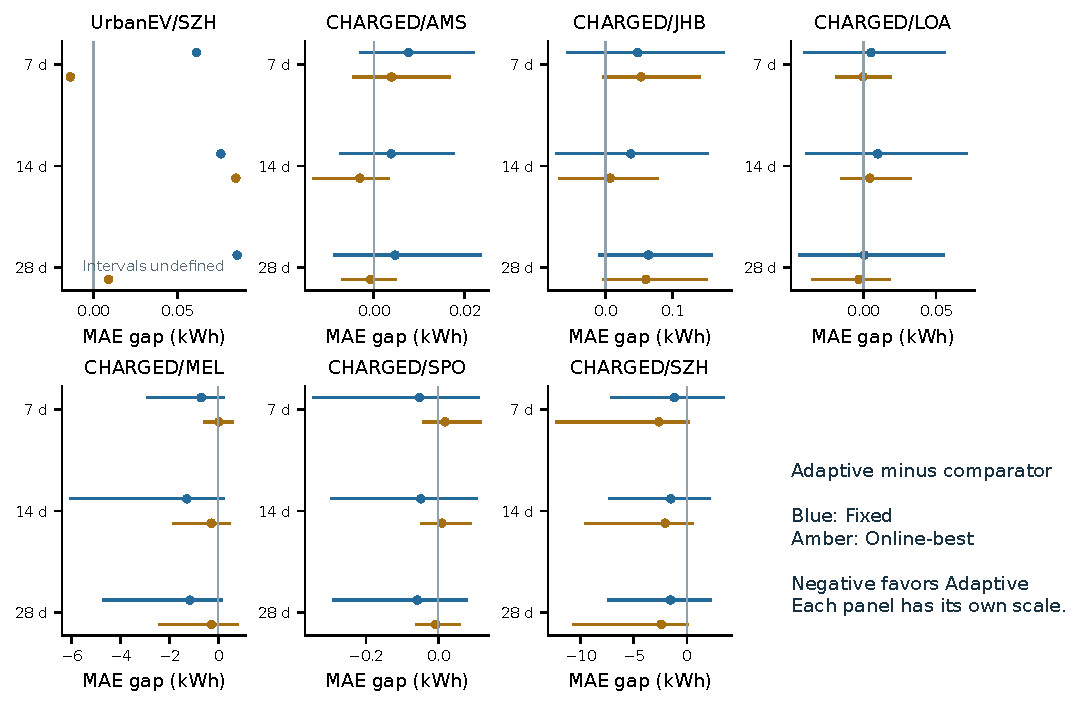
\includegraphics[width=\textwidth]{fig-intervals-v8.pdf}\caption{Adaptive-minus-comparator original-kWh gaps and frozen exploratory 95\% intervals. All finite intervals cross zero. Each panel has its own kWh scale; the scale differs because groups have different demand magnitudes. UrbanEV intervals remain undefined (40/2,000 replicates).}\end{figure}
The bootstrap resamples paired stations and common seven-day circular calendar blocks, conditional on the fixed three-seed average. Undefined replicates are not dropped. Small, possibly colocated cohorts, nonstationarity and lack of simultaneous-comparison adjustment limit interpretation.
\section{Continuation-audit coverage}
Across all histories, finite/new-lower/old-lower/null audit counts are UrbanEV 197/124/73/24; AMS 100/97/3/0; JHB 77/59/18/0; LOA 77/39/38/0; MEL 61/29/32/0; SPO 78/47/31/0; CHARGED/SZH 77/27/50/0. Exact signs include numerical-scale differences. AMS medians are approximately $-3\times10^{-11}$ to $-6\times10^{-11}$ kWh, while MEL/14 has median $+0.1007$ kWh and CHARGED/SZH medians are positive at every history. These clustered records cover exported paired continuations, not the complete switch inventory. The protocol supplies no practical-harm threshold. Full coverage by history is in the audit CSV.


\clearpage\section{Results from a separate implementation}\label{sec:secondary}
A second team implementation completed a separate UrbanEV Final on three IDs (2118, 2534 and 2579), histories 7/14/28 and seeds 7/11/19. It comprises 360 physical jobs; the deterministic Seasonal naive baseline is run once per station--history rather than three times. The IDs are disjoint from the primary UrbanEV cohort, but source states, seeds, head implementations and calibration differ. We therefore retain it as supporting within-track evidence and do not pool it or call it a numerical replication of the primary implementation.

Its principal Adaptive-like method has macro MAE 8.0505, 8.0424 and 7.9156 kWh, compared with Target-only 13.5907, 13.0427 and 12.4014. These are substantial within-track transfer gains, but Fixed (7.9607/7.9523/7.8599) and Online-best (7.9824/7.9494/7.8844) are lower at each history. One station accounts for approximately 83--85\% of the absolute transfer reduction. Component checks do not establish training parity between the implementations; the second track reinforces the need to separate transfer benefit from selector superiority. It is not an additional three-station sample to be appended mechanically to the primary macro average.

\end{document}